\documentclass{article}
\usepackage{amssymb}
\usepackage{color}
\usepackage{listings}
\usepackage{graphicx}
\usepackage{subcaption}
\usepackage{geometry}
\geometry{
a4paper,
total={170mm,257mm},
left=20mm,
top=20mm,
}

\setlength{\parindent}{0em}
\setlength{\parskip}{1em} % length of the spacing

\lstset{ % General setup for the package
    language=Python,
    basicstyle=\small\sffamily,
    numbers=left,
    numberstyle=\tiny,
    frame=tb,
    tabsize=4,
    columns=fixed,
    showstringspaces=false,
    showtabs=false,
    keepspaces,
    commentstyle=\color{red},
    keywordstyle=\color{blue},
    emphstyle=\ttb\color{deepred},    
    stringstyle=\color{deepgreen}
}

\begin{document}
    \title{Navigation and Intelligent Vehicles, Lab session 1 Report}
    \author{Juan Jose Soriano Escobar }
    \maketitle
    \newpage

    \section*{Disclaimer}

    This lab session is developed with Python Instead of Matlab, due to the lack of experience with Matlab
    and because I am more familiar with Python from the previous courses in the Master program. Additionally,
    Python has several libraries that could be easily use to deploy the solution in a web server or in a embedded system.

    On top of Python, I've used numpy library to manipulate multidimensional array objects, and pylab to display the results in graphs. 

    With all that said, I expect to achieve the same results and learn the same concepts as working with Matlab.

    \section{Simulated measurement data}
    

    As  first, before going into the Kalman Filter application  or coding the model itself, I started by creating the measurements
    as was suggested in the Laboratory document \cite{LabManual}. A normal random distributed noise centered in 0.0 with a standard deviation 0.1, 
    for a constant value of 0.26578 voltages.

    The voltages sampled were simulated for 50 measurements using the fragment of code \ref{lst:measurementData}.

    \begin{lstlisting}[language=Python, caption= Measurement data simulation, label={lst:measurementData}]
        import numpy as np

        # for 50 measurements simulated
        iterations = 50

        x = np.full(iterations, 0.26578)
        noise = np.random.normal(0.0, 0.1, iterations) 
        Z = x + noise
    \end{lstlisting}

    \section{Programing the Kalman Filter}

    Following the Kalman Filter logic from the theory, the code is divided in two functions. The first one is the  prediction function for the
    future value of the state value and the error covariance. The function developed for the predictions is presented in the code Listing \ref{lst:prediction}.

    \begin{lstlisting}[language=Python, caption= Prediction Kalman function, label={lst:prediction}]
        def prediction(X, P, A, Q, B, U):
            X = np.dot(A, X) + np.dot(B, U) 
            P = np.dot(A, np.dot(P, A)) + Q 
            return X, P    
    \end{lstlisting}


    The prediction function predict the values of the state value and the error covariance receiving 5 arguments:

    X: The state estimate of the previous step. \\
    P: The state covariance of the previous step. \\
    A: The transition matrix. \\
    Q: The process noise covariance matrix. \\
    B: The input effect matrix. \\
    U: The control input. \\

    With those arguments the new X and P are predicted based on the equations \ref{eq:1} and  \ref{eq:2}.
    \begin{equation} \label{eq:1}
        x(k) = Ax(k - 1) + Bu(k)         
    \end{equation}
    \begin{equation} \label{eq:2}
        P(k) = AP(k - 1)A^T + Q 
    \end{equation}
    Once the prediction is done, it is necessary to update the measurement and verify the error prediction based on the real measured value.
    In this order, the update function presented in the the Listing \ref{lst:update}, receives 6 arguments:

    X: The state estimate. \\
    P: The state covariance. \\
    C: The measurement matrix. \\
    K: The gain or blending value (Kalman gain matrix).\\
    Z: The measurement. \\
    R: The measurement covariance matrix. \\

    \begin{lstlisting}[language=Python, caption= Update Kalman function, label={lst:update}]
        def update(X, P, C, K, Z, R):
            MP = np.dot(C, X) # measurement prediction
            residual = Z - MP 
            MPC = np.dot(C, np.dot(P, C))  + R  # MP covariance
            K = np.dot(P, np.dot(C, MPC**-1)) 
            X = X + np.dot(K, residual) 
            P = P - np.dot(K, np.dot(K, np.dot(MPC, K.T))) 
    
            return (X,P,K) 
    \end{lstlisting}

    To compute the residuals and calculate the gain or blending value K, together with the updated value of the state estimate X and the
    state covariance P. 

    The calculations done in the update function are based on the equation 5, 6 and 7 from \cite{LabManual}. Where MP is the measurement prediction, 'MPC' is the measurement
    prediction covariance and residual is the difference between the measured and predicted value.

    This two functions are enough to apply the Kalman Filter to the specific case of study. Thereafter, a for loop is needed to simulated the
    50 iterations, where the function and update value are going to be implemented as is shown in the section of code \ref{lst:simulationLoop}.

    \begin{lstlisting}[language=Python, caption= Simulation for n amount if iterations, label={lst:simulationLoop}]
        for i in range(1, iterations):    
            # prediction
            X[i], P[i] = prediction(X[i-1], P[i-1], A, Q, B, U)
            # update the values
            X[i], P[i], K[i] = 
                update(X[i-1], P[i-1], C, K[i-1],Z[i-1], R)
    \end{lstlisting}

    At this point, the code is ready to be applied in the the voltage measurement problem.

    \section{Code implementation}

    \subsection{Initial values}
        
    As always in any algorithm or code  to be executed, the first step is to declare the variables with it initial values.
    For this specific problem I have defined:

    A = 1 - The state is a constant. \\
    U = 0 - There is no control input.
    B = 0 - There is no control input. \\
    C = 1 - The noisy measurement is direct. \\
    Q = 10e-5 - Process variance. \\
    R = 0.01 - given from the problem as a constant noise. \\
    X = np.zeros(iterations)  - Initializing voltage estimate the array with the number of iterations.  \\
    P = np.zeros(iterations) - Initializing error estimate the array with the number of iterations. \\
    K = np.zeros(iterations) - gain or blending factor initialization.\\
    ISE = np.zeros(iterations) - Instant Square Error. \\
    MSE = np.zeros(iterations) - Mean Square Error. \\
    x = np.full(iterations, 0.26578) \\
    noise = np.random.normal(0.0, 0.1, iterations) - for 50 measurements simulated. \\
    Z = x + noise

    initial state and error covariance values \\
    X[0] = 0.0 \\
    P[0] = 1.0 \\

    From this point, we define for the given problem the different scenarios to be studied.
    
    \subsection{Simulation for Q = 10e-5 and R = 0.01}
    
    In the figure \ref{fig:simulation1} (a), is visible how the estimate voltage starts with relatively
    large variations in the first 20 iterations and in the ISE (Instant Square Error) in the section (c), 
    but it gradually decrease while the gain value is calculated to filter the signal noise as is visible
    in the section (b) and (d) for the Kalman gain itself and for the MSE (Mean Square Error), respectively.
    Where the MSE in the last iterations is close to 0.01 which is expected from the standard deviation of 
    the noise Gaussian function in the simulated measurements.

    \begin{figure}
        \begin{subfigure} {.5\textwidth}  
            \centering 
            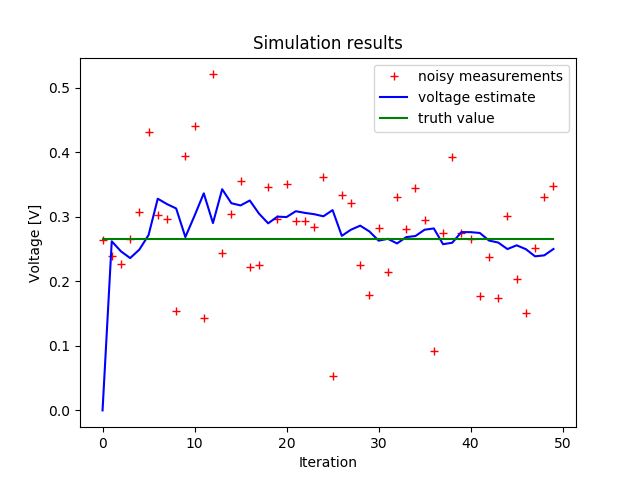
\includegraphics[width=0.8\linewidth]{./img/r01q_.png}
            \caption{Predicted signal from noisy measurements }
        \end{subfigure}
        \begin{subfigure}{.5\textwidth}            
            \centering
            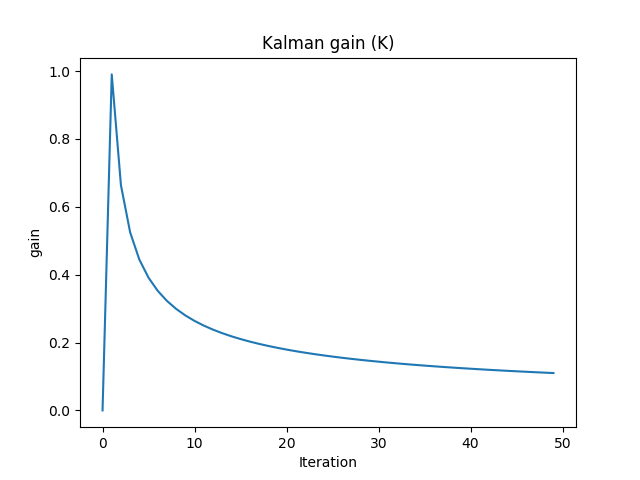
\includegraphics[width=0.8\linewidth]{./img/r01q_K.png}
            \caption{Kalman gain factor}
        \end{subfigure}
        \begin{subfigure} {.5\textwidth}  
            \centering 
            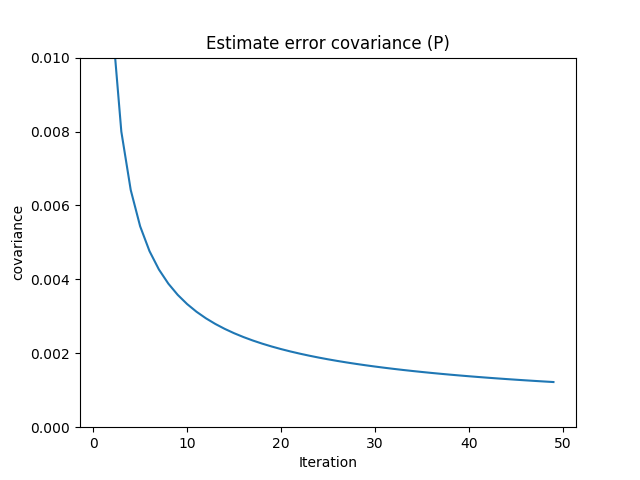
\includegraphics[width=0.8\linewidth]{./img/r01q_P.png}
            \caption{Estimate error covariance}
        \end{subfigure}
        \begin{subfigure}{.5\textwidth}            
            \centering
            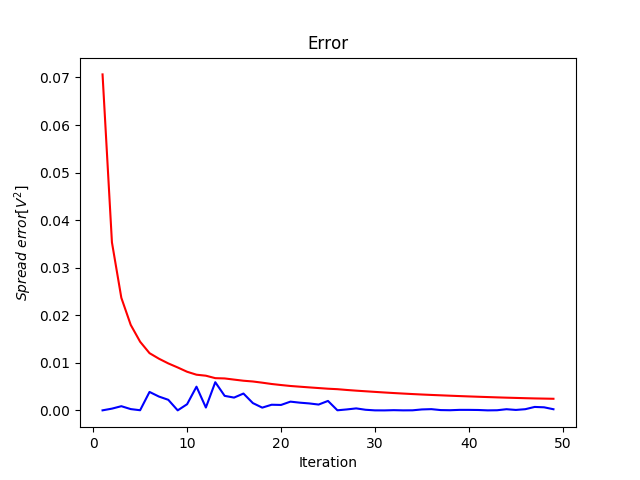
\includegraphics[width=0.8\linewidth]{./img/r01q_E.png}
            \caption{Error measurements MSE (red) and ISE (blue)}
        \end{subfigure}
        \caption{Simulation graph results for R = 0.01 and Q = 10e-5.}
        \label{fig:simulation1}
    \end{figure}
    
    

    Results

    \subsection{Simulation for Q = 10e-5 and R = 0.0001 (R increased on a factor of 1000)} 
    
    When the measurement covariance is decreased by a factor of a thousand (R = 0.0001), it dos not 
    significantly changes the behavior of the prediction, because the R is already smaller than the noise
    in the measurement. As is illustrated in the \ref{fig:simulation2} the values and the predictions is nearly
    the same as in the previous scenario. The only difference is the decimals precision of P,  consequence
    of the equation (5) from \cite{LabManual} where R is added to K to later on update P.

    \begin{figure}
        \begin{subfigure} {.5\textwidth}  
            \centering 
            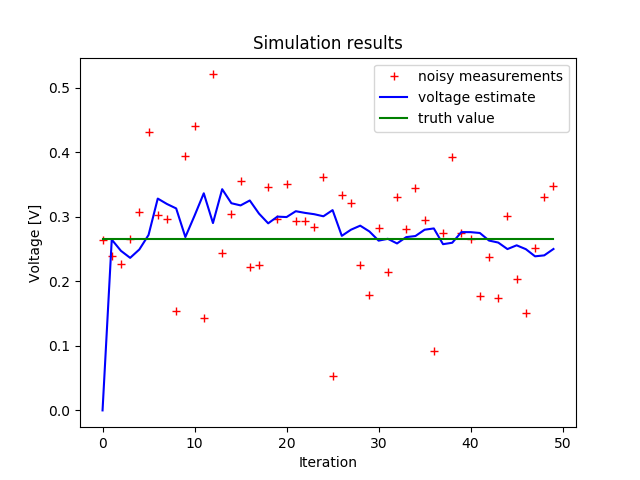
\includegraphics[width=0.8\linewidth]{./img/r00001q_.png}
            \caption{Predicted signal from noisy measurements }
        \end{subfigure}
        \begin{subfigure}{.5\textwidth}            
            \centering
            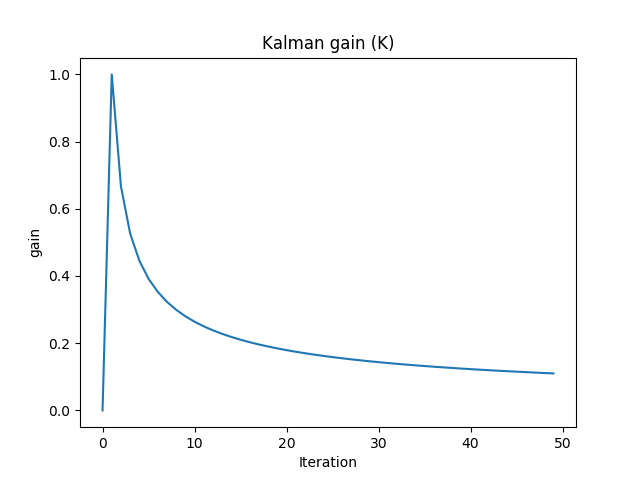
\includegraphics[width=0.8\linewidth]{./img/r00001q_K.png}
            \caption{Kalman gain factor}
        \end{subfigure}
        \begin{subfigure} {.5\textwidth}  
            \centering 
            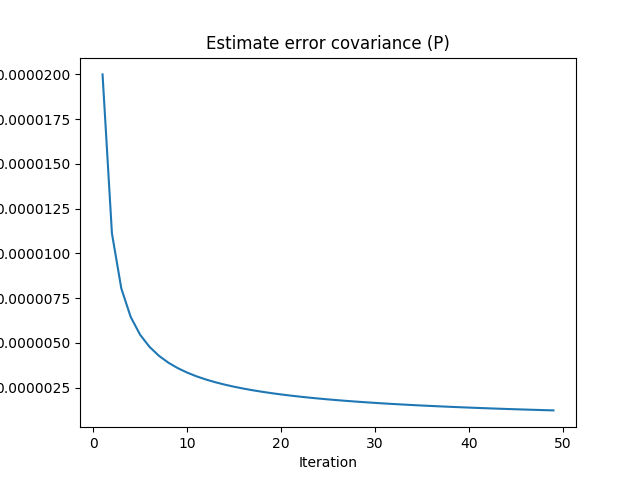
\includegraphics[width=0.8\linewidth]{./img/r00001q_P.png}
            \caption{Estimate error covariance}
        \end{subfigure}
        \begin{subfigure}{.5\textwidth}            
            \centering
            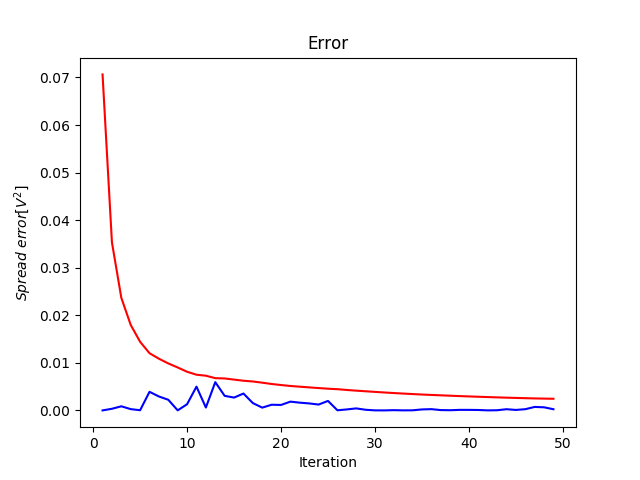
\includegraphics[width=0.8\linewidth]{./img/r00001q_E.png}
            \caption{Error measurements MSE (red) and ISE (blue)}
        \end{subfigure}
        \caption{Simulation graph results for R = 0.0001 and Q = 10e-5.}
        \label{fig:simulation2}
    \end{figure}

    \subsection{Simulation for Q = 10e-5 and R = 10 (R decreased on a factor of 1000)}

    On the other hand, when R is increased by a factor of a 1000 (R = 10) the results drastically changes for
    all the studies graphs as is presented on the \ref{fig:simulation3}. It starts by the measurement variance
    prediction incrementing by 10, which later slows slows down the Kalman gain due to R which is in the divisor
    of the Kalman gain.
    
    This behavior consequently reduces the update form P value where K is involve in the equation (7) form \cite{LabManual},
    taking more iterations to filter the noise and to reach the predictions precision obtained in the 
    previous scenarios.


    \begin{figure}
        \begin{subfigure} {.5\textwidth}  
            \centering 
            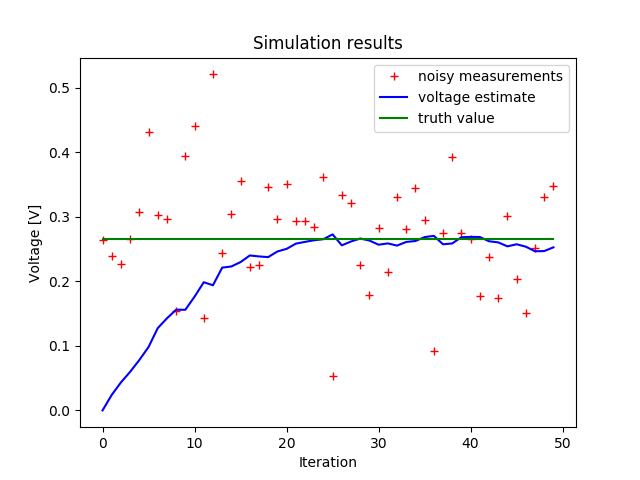
\includegraphics[width=0.8\linewidth]{./img/r10q_.png}
            \caption{Predicted signal from noisy measurements }
        \end{subfigure}
        \begin{subfigure}{.5\textwidth}            
            \centering
            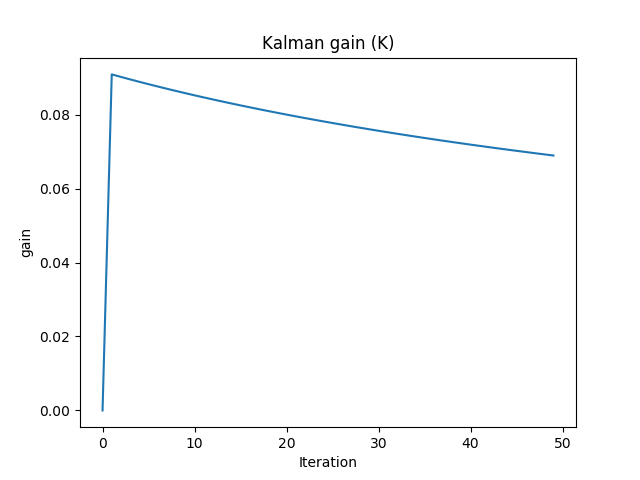
\includegraphics[width=0.8\linewidth]{./img/r10q_K.png}
            \caption{Kalman gain factor}
        \end{subfigure}
        \begin{subfigure} {.5\textwidth}  
            \centering 
            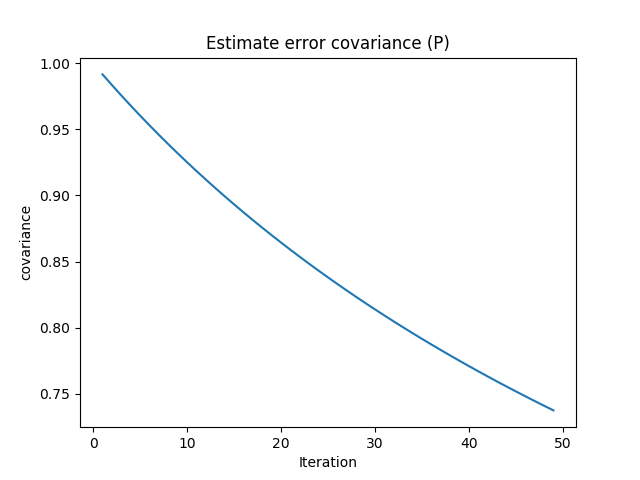
\includegraphics[width=0.8\linewidth]{./img/r10q_P.png}
            \caption{Estimate error covariance}
        \end{subfigure}
        \begin{subfigure}{.5\textwidth}            
            \centering
            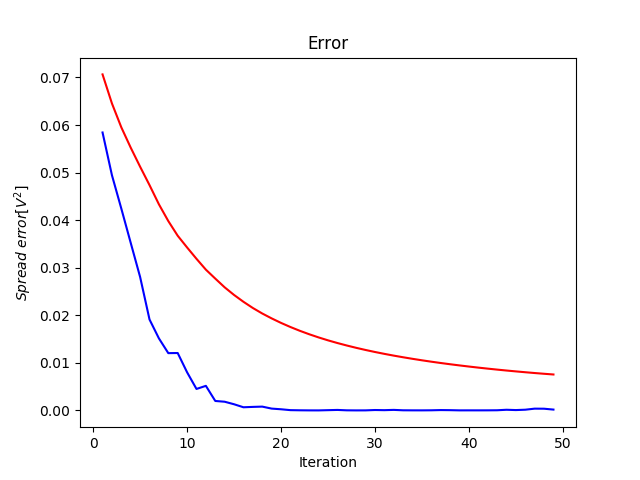
\includegraphics[width=0.8\linewidth]{./img/r10q_E.png}
            \caption{Error measurements MSE (red) and ISE (blue)}
        \end{subfigure}
        \caption{Simulation graph results for R = 10 and Q = 10e-5.}
        \label{fig:simulation3}
    \end{figure}
    

    \subsection{Simulation for Q = 10e-8 and R = 0.01 (Q increased on a factor of 1000)}
    
    Similarly to the scenario with R = 0.0001m when Q is decreased by a factor of a thousand it does not 
    affect in a significantly results as is visible in the figure \ref{fig:simulation4}. In this case
    again, P changes the decimal precision because Q is directly add to the prediction of P in the equation 
    \ref{eq:2}.

    \begin{figure}
        \begin{subfigure} {.5\textwidth}  
            \centering 
            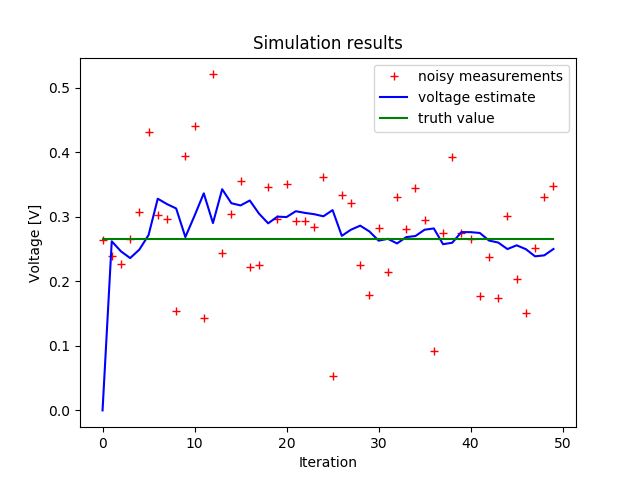
\includegraphics[width=0.8\linewidth]{./img/r01q-8_.png}
            \caption{Predicted signal from noisy measurements }
        \end{subfigure}
        \begin{subfigure}{.5\textwidth}            
            \centering
            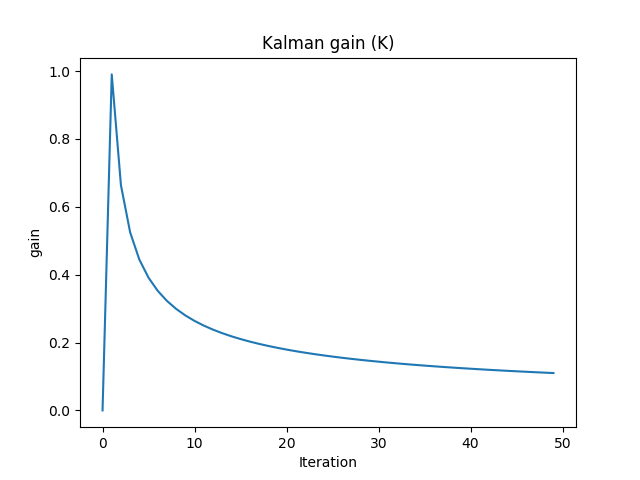
\includegraphics[width=0.8\linewidth]{./img/r01q-8_K.png}
            \caption{Kalman gain factor}
        \end{subfigure}
        \begin{subfigure} {.5\textwidth}  
            \centering 
            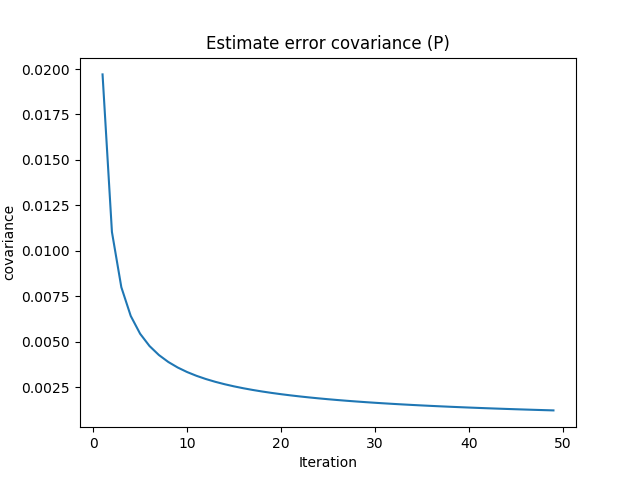
\includegraphics[width=0.8\linewidth]{./img/r01q-8_P.png}
            \caption{Estimate error covariance}
        \end{subfigure}
        \begin{subfigure}{.5\textwidth}            
            \centering
            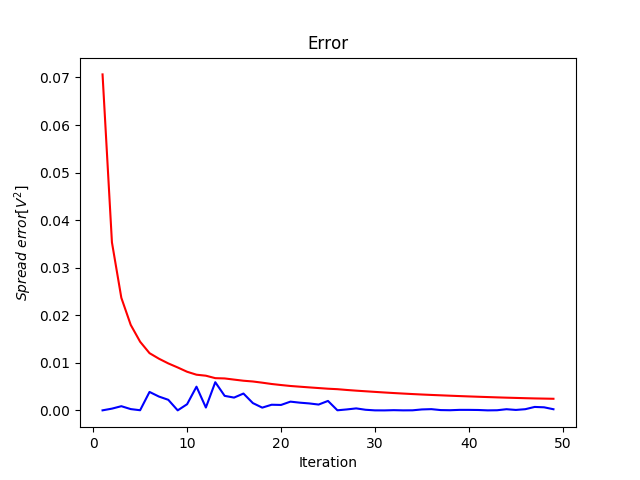
\includegraphics[width=0.8\linewidth]{./img/r01q-8_E.png}
            \caption{Error measurements MSE (red) and ISE (blue)}
        \end{subfigure}
        \caption{Simulation graph results for R = 0.01 and Q = 10e-8.}
        \label{fig:simulation4}
    \end{figure}   

    \subsection{Simulation for Q = 10e-8 and R = 0.01 (Q decreased on a factor of 1000)}
    
    Similarly to the scenario with R = 0.0001m when Q is decreased by a factor of a thousand it does not 
    affect in a significantly results as is visible in the figure \ref{fig:simulation4}. In this case
    again, P changes the decimal precision because Q is directly add to the prediction of P in the equation 
    \ref{eq:2}.

    \begin{figure}
        \begin{subfigure} {.5\textwidth}  
            \centering 
            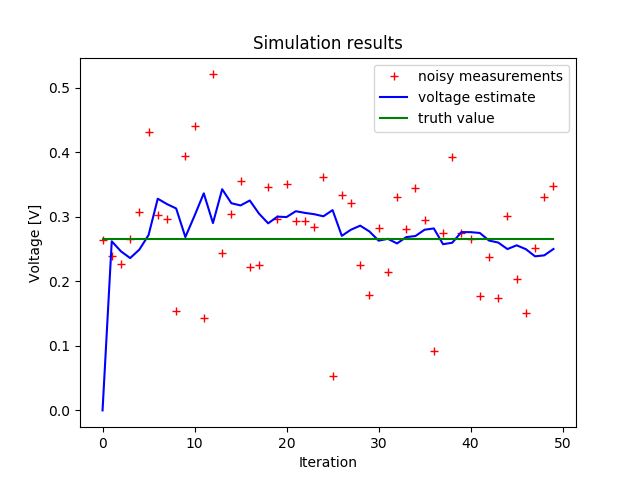
\includegraphics[width=0.8\linewidth]{./img/r01q-2_.png}
            \caption{Predicted signal from noisy measurements }
        \end{subfigure}
        \begin{subfigure}{.5\textwidth}            
            \centering
            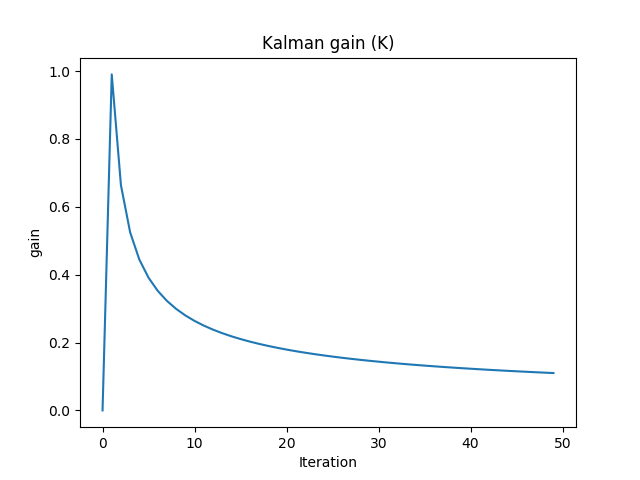
\includegraphics[width=0.8\linewidth]{./img/r01q-2_K.png}
            \caption{Kalman gain factor}
        \end{subfigure}
        \begin{subfigure} {.5\textwidth}  
            \centering 
            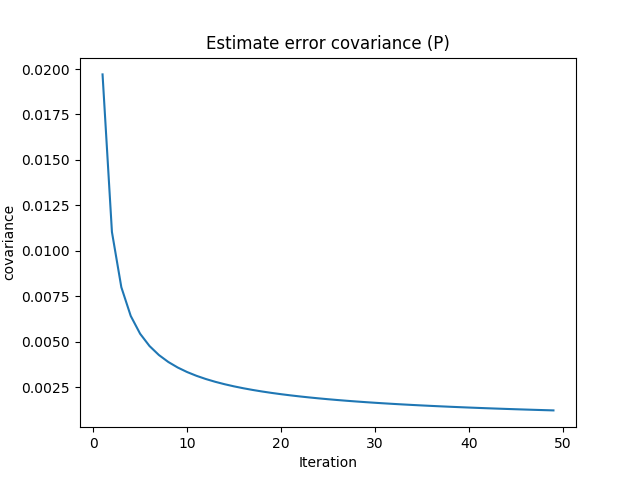
\includegraphics[width=0.8\linewidth]{./img/r01q-2_P.png}
            \caption{Estimate error covariance}
        \end{subfigure}
        \begin{subfigure}{.5\textwidth}            
            \centering
            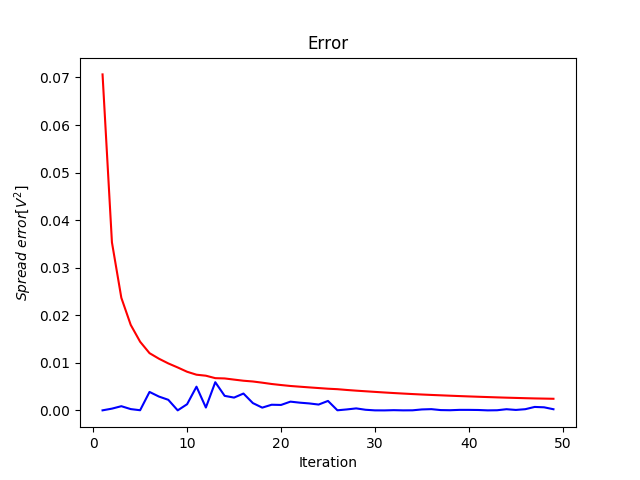
\includegraphics[width=0.8\linewidth]{./img/r01q-2_E.png}
            \caption{Error measurements MSE (red) and ISE (blue)}
        \end{subfigure}
        \caption{Simulation graph results for R = 0.01 and Q = 10e-2.}
        \label{fig:simulation5}
    \end{figure}

    \subsection{Simulation for Q = 10e-2 and R = 0.01 (Q decreased on a factor of 1000)}
    
    As presented in  the previous scenario, the results are almost the same due to a small process covariance close to zero.
    For this reason I avoided to presented the graph result.


    \subsection{What if the noise measurement is no longer zero mean?}
    
        All the results will be x value deviated from the truth voltage value. As is visible in
        the \ref{fig:simulation6} (a), the Filter will keep on trying to reduced the noise but 
        converging to ground truth plus the deviation in the mean (0.5 for the presented case). This will
        also going to affect the error indicator MSE and ISE (d), proving once more that the measurement are deviated from
        the original value. 

        To avoid this kind of results, before of applying the filter is recommended to normalize the measurements with the
        expected value.
    
        \begin{figure}
            \begin{subfigure} {.5\textwidth}  
                \centering 
                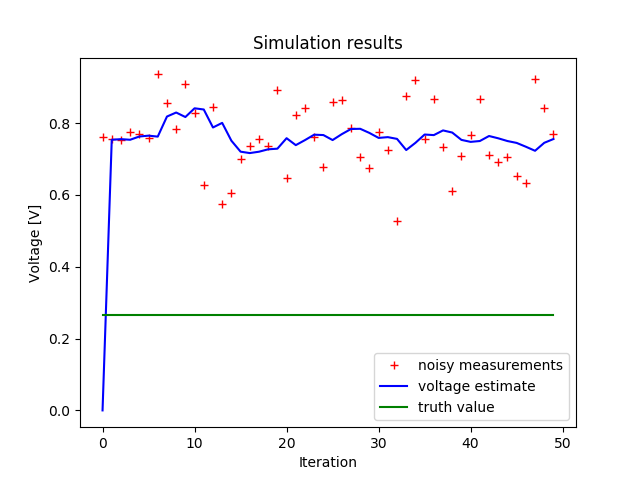
\includegraphics[width=0.8\linewidth]{./img/nc_.png}
                \caption{Predicted signal from noisy measurements }
            \end{subfigure}
            \begin{subfigure}{.5\textwidth}            
                \centering
                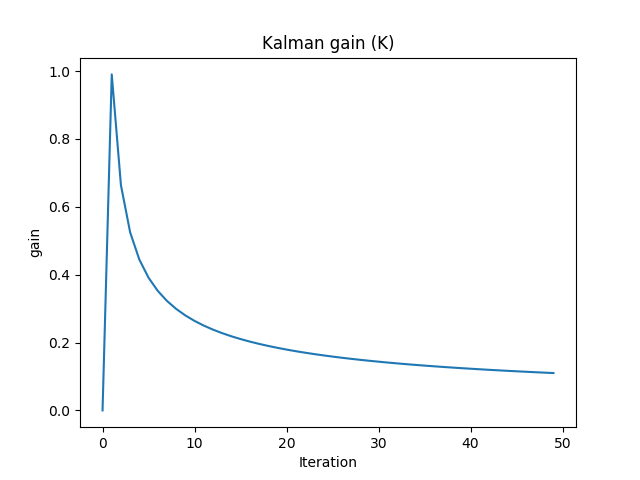
\includegraphics[width=0.8\linewidth]{./img/nc_K.png}
                \caption{Kalman gain factor}
            \end{subfigure}
            \begin{subfigure} {.5\textwidth}  
                \centering 
                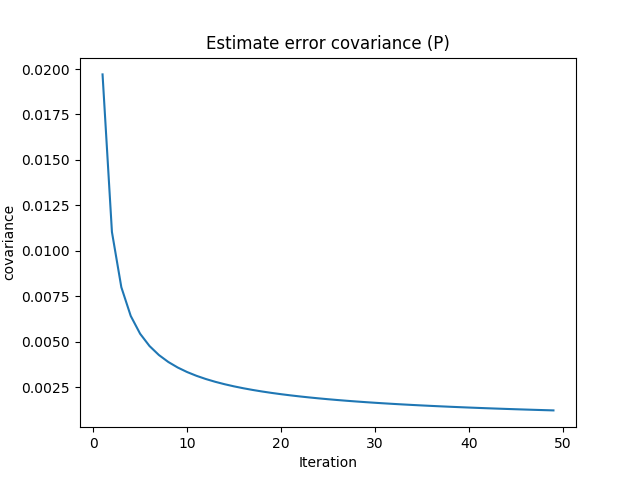
\includegraphics[width=0.8\linewidth]{./img/nc_P.png}
                \caption{Estimate error covariance}
            \end{subfigure}
            \begin{subfigure}{.5\textwidth}            
                \centering
                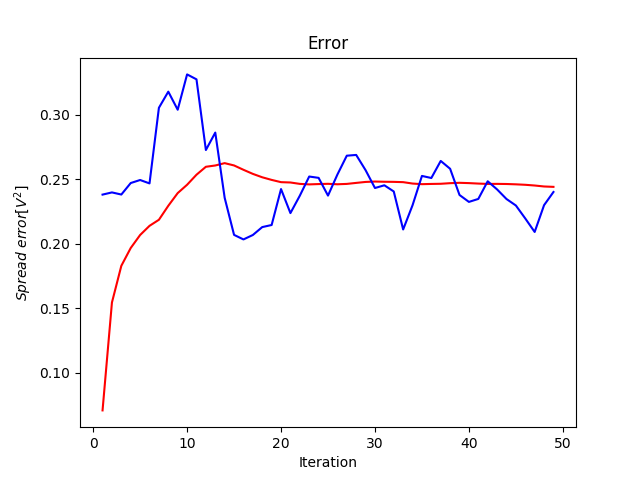
\includegraphics[width=0.8\linewidth]{./img/nc_E.png}
                \caption{Error measurements MSE (red) and ISE (blue)}
            \end{subfigure}
            \caption{Simulation with no zero center noise N(0.5, 0.01).}
            \label{fig:simulation6}
        \end{figure}
    
    \subsection{What happens if you change the initial value of the error covariance P?}
    
    I tried P with different values end the result did not changed much for big values or values bigger than 0.1 in general.
    The first critical value is when P = 0. In the \ref{fig:simulation7} (a) is visible how the filter is not able to estimate the
    voltage. This is the result of an indetermination in the K gain in the equation (7) from \cite{LabManual},
    where K is divided by P. 

    With a negative value of P, the covariance will keep on decreasing as  in visible in \ref{fig:simulation7} (c)
    Increasing the error of the prediction exponentially. This is explained by the negative divisor in the K gain value.
    
    On the other hand for a P smaller than the noise and close to R, the figure \ref{fig:simulation7} (b),
    presents similar Results as the simulation with R = 10. This result is expected, because in the K gain factor R is 
    basically increased in a factor of a thousand compared with the value of P. Where K could be reduced to 
    K = P / (P + R).

    In accordance to this results, could be a value from ( 0, + inf.) and preferably higher than the estimate of
    the measurement variance R.

    \begin{figure}
        \begin{subfigure} {.3\textwidth}  
            \centering 
            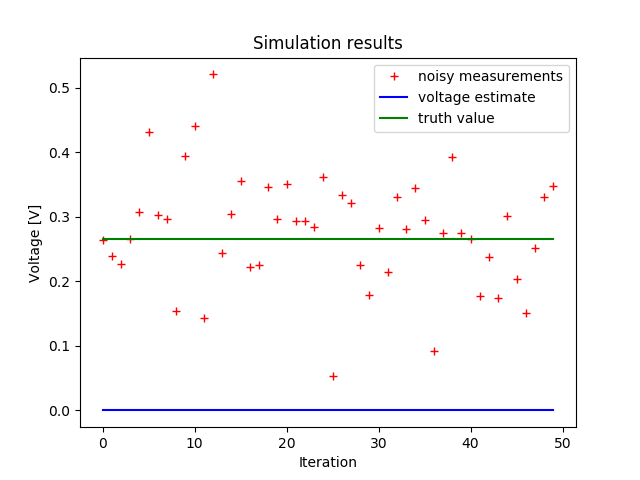
\includegraphics[width=0.8\linewidth]{./img/P0_.png}
            \caption{P = 0 }
        \end{subfigure}
        \begin{subfigure}{.3\textwidth}            
            \centering
            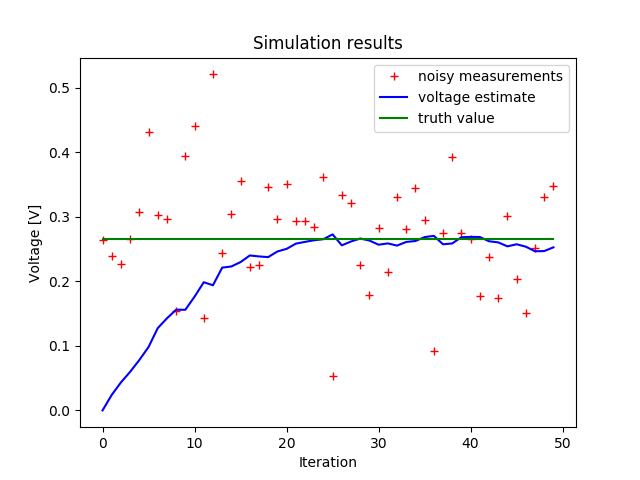
\includegraphics[width=0.8\linewidth]{./img/P001_.png}
            \caption{P = 0.001}
        \end{subfigure}    
        \begin{subfigure} {.3\textwidth}         
            \centering
            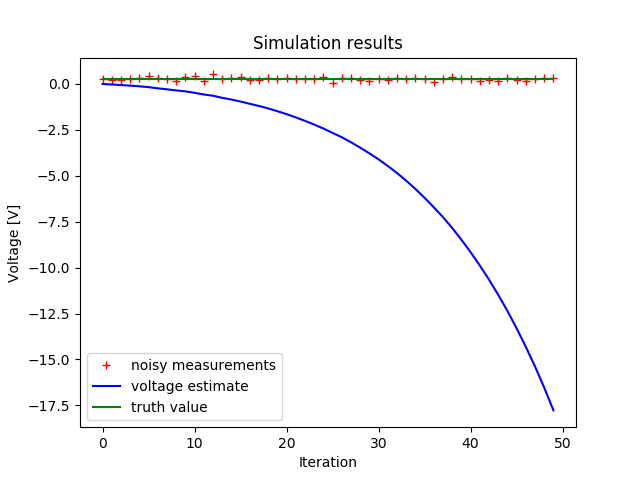
\includegraphics[width=0.8\linewidth]{./img/Pneg.png}
            \caption{P = -0.001}
        \end{subfigure}
        \caption{Simulation for P = 0, P =  0.001 and P = -0.001}
        \label{fig:simulation7}
    \end{figure}
    

    \subsection{Does the value of the Kalman gain K contain information?}

    The K gain is and important parameter in the Kalman Filter because it shows the relationship
    between the magnitude of the input to the magnitude of the output signal. In other words, it determines
    the relative difference of the voltage in response to a change in the controller output, which is constant 
    for this case of study.

    \subsection{Are there any other parameters that influence your KF?}

    The Kalman filter depends directly on P (error estimate) and R (estimate of measurement variance) and indirectly
    on Q which is th process variance use to predict the value of P.

    \bibliography{report}
    \bibliographystyle{ieeetr}
    \nocite{*}
    % Implementation of Kalman Filter with Python Language ... pdf
    % http://scottlobdell.me/2014/08/kalman-filtering-python-reading-sensor-input/

\end{document}
